As we will see in the following sections, the state representation of the
environment is a crucial aspect of the learning process. If the state
representation is too large, the learning process will be slow, and the agent
will require more samples to learn. On the other hand, if the state
representation is too small, the agent will not be able to learn the
environment's dynamics.

We will come to find that training a \gls{cnn} on the \gls{rgb}-state is
computationally expensive, and the agent will require a more samples to learn
from the environment then feasible for this project. To mitigate this issue, we
will scale down the state representation to a more manageable size. For this
scaled-down state representation, we will consider two different
representations: the \gls{rgb}-state and the grayscale-state.

\subsubsection{RGB-state}\label{sec:environment-state-representation-scaling-rgb-state}
As mentioned before, the \gls{rgb} state is the default representation of the
Q*bert Atari environment. The \gls{rgb} state is a three-dimensional tensor
where each dimension represents the red, green, and blue channels of the
environment, and has a size of 210x160x3, which is a large representation of
the environment. The \gls{rgb} state and its scaled down version are shown in
\cref{fig:rgb-state}.

\begin{figure}[H]
    \centering
    \begin{subfigure}{0.45\textwidth}
        \centering
        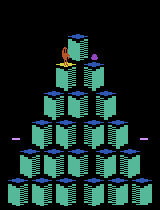
\includegraphics[width=\textwidth]{img/rgb-full-purple.png}
        \caption{Full state representation.}
        \label{fig:rgb-full}
    \end{subfigure}
    \begin{subfigure}{0.45\textwidth}
        \centering
        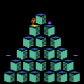
\includegraphics[width=\textwidth]{img/rgb-84x84-purple.png}
        \caption{84x84 state representation.}
        \label{fig:rgb-84x84}
    \end{subfigure}
    \caption{RGB state representation.}
    \label{fig:rgb-state}
\end{figure}

As we see in \cref{fig:rgb-full}, the scaled down version of the \gls{rgb}
state, as shown in \cref{fig:rgb-84x84}, keeps the main features of the
environment, such as the platforms, the enemies, and the player.

\subsubsection{Grayscale-state}\label{sec:environment-state-representation-scaling-grayscale-state}
The grayscaled state is a two-dimensional tensor where each dimension
represents the height and width of the environment, and has a size of 210x160.
The reason for using a grayscaled state is to reduce the complexity of the
environment representation, as the \gls{rgb} state has a large size. This
reduction in size is created by merging the three channels of the \gls{rgb}
state into a single channel, which results in a smaller representation of the
environment. The grayscaled state and its scaled down version are shown in
\cref{fig:gray-state}.

\begin{figure}[H]
    \centering
    \begin{subfigure}{0.45\textwidth}
        \centering
        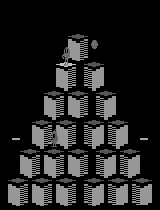
\includegraphics[width=\textwidth]{img/gray-full-purple-sam.png}
        \caption{Full state representation.}
        \label{fig:rgb-full}
    \end{subfigure}
    \begin{subfigure}{0.45\textwidth}
        \centering
        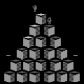
\includegraphics[width=\textwidth]{img/gray-84x84-sam.png}
        \caption{84x84 state representation.}
        \label{fig:rgb-84x84}
    \end{subfigure}
    \caption{RGB state representation.}
    \label{fig:rgb-state}
\end{figure}

As we see in \cref{fig:rgb-full}, the scaled down version of the grayscaled
state, as shown in \cref{fig:rgb-84x84}, keeps the main features of the
environment, such as the platforms, the enemies, and the player. One point of
concern is that the grayscaled state may lose some information that could be
important to the agent, such as the difference in colour of the balls. The
environment contains two types of balls, purple and green, which have opposite
effects on the player. The green ball increases the player's score, while the
purple ball decreases the player's score. The grayscaled values of these
balls are extremely close (103 and 107). However, the agent should be able to
distinguish between these two types of balls to make the best decisions.

Seeing as the grayscaled state should be able to represent the environment
without losing important information, we will use the grayscaled state in our
experiments. We will also use the scaled down version of the grayscaled state
to reduce the complexity of the environment representation.